\documentclass[]{article}
\usepackage{lmodern}
\usepackage{amssymb,amsmath}
\usepackage{ifxetex,ifluatex}
\usepackage{fixltx2e} % provides \textsubscript
\ifnum 0\ifxetex 1\fi\ifluatex 1\fi=0 % if pdftex
  \usepackage[T1]{fontenc}
  \usepackage[utf8]{inputenc}
\else % if luatex or xelatex
  \ifxetex
    \usepackage{mathspec}
    \usepackage{xltxtra,xunicode}
  \else
    \usepackage{fontspec}
  \fi
  \defaultfontfeatures{Mapping=tex-text,Scale=MatchLowercase}
  \newcommand{\euro}{€}
\fi
% use upquote if available, for straight quotes in verbatim environments
\IfFileExists{upquote.sty}{\usepackage{upquote}}{}
% use microtype if available
\IfFileExists{microtype.sty}{%
\usepackage{microtype}
\UseMicrotypeSet[protrusion]{basicmath} % disable protrusion for tt fonts
}{}
\ifxetex
  \usepackage[setpagesize=false, % page size defined by xetex
              unicode=false, % unicode breaks when used with xetex
              xetex]{hyperref}
\else
  \usepackage[unicode=true]{hyperref}
\fi
\usepackage[usenames,dvipsnames]{color}
\hypersetup{breaklinks=true,
            bookmarks=true,
            pdfauthor={},
            pdftitle={},
            colorlinks=true,
            citecolor=blue,
            urlcolor=blue,
            linkcolor=magenta,
            pdfborder={0 0 0}}
\urlstyle{same}  % don't use monospace font for urls
\usepackage{color}
\usepackage{fancyvrb}
\newcommand{\VerbBar}{|}
\newcommand{\VERB}{\Verb[commandchars=\\\{\}]}
\DefineVerbatimEnvironment{Highlighting}{Verbatim}{commandchars=\\\{\}}
% Add ',fontsize=\small' for more characters per line
\newenvironment{Shaded}{}{}
\newcommand{\KeywordTok}[1]{\textcolor[rgb]{0.00,0.44,0.13}{\textbf{{#1}}}}
\newcommand{\DataTypeTok}[1]{\textcolor[rgb]{0.56,0.13,0.00}{{#1}}}
\newcommand{\DecValTok}[1]{\textcolor[rgb]{0.25,0.63,0.44}{{#1}}}
\newcommand{\BaseNTok}[1]{\textcolor[rgb]{0.25,0.63,0.44}{{#1}}}
\newcommand{\FloatTok}[1]{\textcolor[rgb]{0.25,0.63,0.44}{{#1}}}
\newcommand{\ConstantTok}[1]{\textcolor[rgb]{0.53,0.00,0.00}{{#1}}}
\newcommand{\CharTok}[1]{\textcolor[rgb]{0.25,0.44,0.63}{{#1}}}
\newcommand{\SpecialCharTok}[1]{\textcolor[rgb]{0.25,0.44,0.63}{{#1}}}
\newcommand{\StringTok}[1]{\textcolor[rgb]{0.25,0.44,0.63}{{#1}}}
\newcommand{\VerbatimStringTok}[1]{\textcolor[rgb]{0.25,0.44,0.63}{{#1}}}
\newcommand{\SpecialStringTok}[1]{\textcolor[rgb]{0.73,0.40,0.53}{{#1}}}
\newcommand{\ImportTok}[1]{{#1}}
\newcommand{\CommentTok}[1]{\textcolor[rgb]{0.38,0.63,0.69}{\textit{{#1}}}}
\newcommand{\DocumentationTok}[1]{\textcolor[rgb]{0.73,0.13,0.13}{\textit{{#1}}}}
\newcommand{\AnnotationTok}[1]{\textcolor[rgb]{0.38,0.63,0.69}{\textbf{\textit{{#1}}}}}
\newcommand{\CommentVarTok}[1]{\textcolor[rgb]{0.38,0.63,0.69}{\textbf{\textit{{#1}}}}}
\newcommand{\OtherTok}[1]{\textcolor[rgb]{0.00,0.44,0.13}{{#1}}}
\newcommand{\FunctionTok}[1]{\textcolor[rgb]{0.02,0.16,0.49}{{#1}}}
\newcommand{\VariableTok}[1]{\textcolor[rgb]{0.10,0.09,0.49}{{#1}}}
\newcommand{\ControlFlowTok}[1]{\textcolor[rgb]{0.00,0.44,0.13}{\textbf{{#1}}}}
\newcommand{\OperatorTok}[1]{\textcolor[rgb]{0.40,0.40,0.40}{{#1}}}
\newcommand{\BuiltInTok}[1]{{#1}}
\newcommand{\ExtensionTok}[1]{{#1}}
\newcommand{\PreprocessorTok}[1]{\textcolor[rgb]{0.74,0.48,0.00}{{#1}}}
\newcommand{\AttributeTok}[1]{\textcolor[rgb]{0.49,0.56,0.16}{{#1}}}
\newcommand{\RegionMarkerTok}[1]{{#1}}
\newcommand{\InformationTok}[1]{\textcolor[rgb]{0.38,0.63,0.69}{\textbf{\textit{{#1}}}}}
\newcommand{\WarningTok}[1]{\textcolor[rgb]{0.38,0.63,0.69}{\textbf{\textit{{#1}}}}}
\newcommand{\AlertTok}[1]{\textcolor[rgb]{1.00,0.00,0.00}{\textbf{{#1}}}}
\newcommand{\ErrorTok}[1]{\textcolor[rgb]{1.00,0.00,0.00}{\textbf{{#1}}}}
\newcommand{\NormalTok}[1]{{#1}}
\usepackage{graphicx,grffile}
\makeatletter
\def\maxwidth{\ifdim\Gin@nat@width>\linewidth\linewidth\else\Gin@nat@width\fi}
\def\maxheight{\ifdim\Gin@nat@height>\textheight\textheight\else\Gin@nat@height\fi}
\makeatother
% Scale images if necessary, so that they will not overflow the page
% margins by default, and it is still possible to overwrite the defaults
% using explicit options in \includegraphics[width, height, ...]{}
\setkeys{Gin}{width=\maxwidth,height=\maxheight,keepaspectratio}
\setlength{\parindent}{0pt}
\setlength{\parskip}{6pt plus 2pt minus 1pt}
\setlength{\emergencystretch}{3em}  % prevent overfull lines
\providecommand{\tightlist}{%
  \setlength{\itemsep}{0pt}\setlength{\parskip}{0pt}}
\setcounter{secnumdepth}{0}

\date{}

% Redefines (sub)paragraphs to behave more like sections
\ifx\paragraph\undefined\else
\let\oldparagraph\paragraph
\renewcommand{\paragraph}[1]{\oldparagraph{#1}\mbox{}}
\fi
\ifx\subparagraph\undefined\else
\let\oldsubparagraph\subparagraph
\renewcommand{\subparagraph}[1]{\oldsubparagraph{#1}\mbox{}}
\fi

\begin{document}

\section{A minimal R Markdown
example}\label{a-minimal-r-markdown-example}

\begin{Shaded}
\begin{Highlighting}[]
\CommentTok{# this is a comment}
\CommentTok{# this will run inside an R environment if you remove the # before the ?}
\CommentTok{# ?mean}
\CommentTok{# generic help built into R about the mean function}
\CommentTok{# stats'y language}
\end{Highlighting}
\end{Shaded}

everything in R is a vector (or series of values) x =
{[}x1,x2,x3,\ldots{}xn{]}

\subsection{data types}\label{data-types}

\begin{itemize}
\tightlist
\item
  vector
\item
  matrix (2 dimensional vector of the same data type)
\item
  data.frame (2 dimensional vector of different data types)
\item
  list - arbitrary data types, contain anything
\end{itemize}

some functions need data.frame, other matrices or lists, you must
convert

in R, observations (samples) are typically in rows, and variables
(genes, OTUs, etc) are in columns

lets make 3 vectors and examine them These functions generate random
numbers and we can get summary statistics of them.

```\{r, eval=TRUE\} \# all functions in R contain their arguments in ()
\# all subsetting uses {[}{]} \# all programming is inside \{\}

\section{\textless{}- assignment}\label{assignment}

\section{c() concatenation function}\label{c-concatenation-function}

\section{runif() random uniform function to generate pseudo random
numbers}\label{runif-random-uniform-function-to-generate-pseudo-random-numbers}

x \textless{}- c(runif(10, 0,10)) y \textless{}- c(runif(10,2,10)) z
\textless{}- c(runif(10,0,5))

\begin{verbatim}
# what is the mean value of vector x?

mean(x)
\end{verbatim}

\begin{Shaded}
\begin{Highlighting}[]
\NormalTok{## [1] 3.992126}
\end{Highlighting}
\end{Shaded}

\begin{Shaded}
\begin{Highlighting}[]
\KeywordTok{mean}\NormalTok{(y)}
\end{Highlighting}
\end{Shaded}

\begin{verbatim}
## [1] 5.970781
\end{verbatim}

\begin{Shaded}
\begin{Highlighting}[]
\KeywordTok{mean}\NormalTok{(z)}
\end{Highlighting}
\end{Shaded}

\begin{verbatim}
## [1] 2.669965
\end{verbatim}

\begin{Shaded}
\begin{Highlighting}[]
\KeywordTok{summary}\NormalTok{(x)}
\end{Highlighting}
\end{Shaded}

\begin{verbatim}
##    Min. 1st Qu.  Median    Mean 3rd Qu.    Max. 
##  0.1318  2.5510  3.9230  3.9920  4.9360  8.4270
\end{verbatim}

\begin{Shaded}
\begin{Highlighting}[]
\CommentTok{# we can subset from a vector}
\KeywordTok{summary}\NormalTok{(x)[}\DecValTok{2}\NormalTok{]}
\end{Highlighting}
\end{Shaded}

\begin{verbatim}
## 1st Qu. 
##   2.551
\end{verbatim}

Now we can convert xyz into a matrix using cbind. What does the rbind()
function do?

\begin{Shaded}
\begin{Highlighting}[]
\NormalTok{xyz <-}\StringTok{ }\KeywordTok{cbind}\NormalTok{(x,y,z)}
\KeywordTok{dim}\NormalTok{(xyz)}
\end{Highlighting}
\end{Shaded}

\begin{verbatim}
## [1] 10  3
\end{verbatim}

\begin{Shaded}
\begin{Highlighting}[]
\KeywordTok{is.matrix}\NormalTok{(xyz)}
\end{Highlighting}
\end{Shaded}

\begin{verbatim}
## [1] TRUE
\end{verbatim}

\begin{Shaded}
\begin{Highlighting}[]
\KeywordTok{is.data.frame}\NormalTok{(xyz)}
\end{Highlighting}
\end{Shaded}

\begin{verbatim}
## [1] FALSE
\end{verbatim}

\begin{Shaded}
\begin{Highlighting}[]
\CommentTok{# or subset xyz matrix to third column and rows 1 to 5}

\NormalTok{xyz[}\DecValTok{1}\NormalTok{:}\DecValTok{5}\NormalTok{,}\DecValTok{3}\NormalTok{]}
\end{Highlighting}
\end{Shaded}

\begin{verbatim}
## [1] 3.646010 2.415433 1.043958 2.155368 1.492127
\end{verbatim}

\begin{Shaded}
\begin{Highlighting}[]
\CommentTok{# we can make xyz into a data.frame}
\NormalTok{df.xyz <-}\StringTok{ }\KeywordTok{as.data.frame}\NormalTok{(xyz)}

\CommentTok{# and examine the structure}
\KeywordTok{str}\NormalTok{(xyz)}
\end{Highlighting}
\end{Shaded}

\begin{verbatim}
##  num [1:10, 1:3] 7.83 2.71 8.43 2.5 4.03 ...
##  - attr(*, "dimnames")=List of 2
##   ..$ : NULL
##   ..$ : chr [1:3] "x" "y" "z"
\end{verbatim}

\begin{Shaded}
\begin{Highlighting}[]
\KeywordTok{str}\NormalTok{(df.xyz)}
\end{Highlighting}
\end{Shaded}

\begin{verbatim}
## 'data.frame':    10 obs. of  3 variables:
##  $ x: num  7.83 2.71 8.43 2.5 4.03 ...
##  $ y: num  9.26 5.82 9.13 5.28 3.68 ...
##  $ z: num  3.65 2.42 1.04 2.16 1.49 ...
\end{verbatim}

we can make random data drawn from a normal distribution using the rnorm
function

\begin{Shaded}
\begin{Highlighting}[]
\CommentTok{# drawing 10 values with a mean of 5 and a standard deviation of 2}
\NormalTok{xn <-}\StringTok{ }\KeywordTok{rnorm}\NormalTok{(}\DecValTok{10}\NormalTok{,}\DecValTok{5}\NormalTok{,}\DecValTok{2}\NormalTok{)}
\end{Highlighting}
\end{Shaded}

We can explore by examining the data graphically using either boxplots
or stripcharts

\begin{Shaded}
\begin{Highlighting}[]
\CommentTok{# generates a boxplot: http://flowingdata.com/2008/02/15/how-to-read-and-use-a-box-and-whisker-plot/}
\KeywordTok{boxplot}\NormalTok{(x,y,z)}
\end{Highlighting}
\end{Shaded}

\begin{figure}[htbp]
\centering
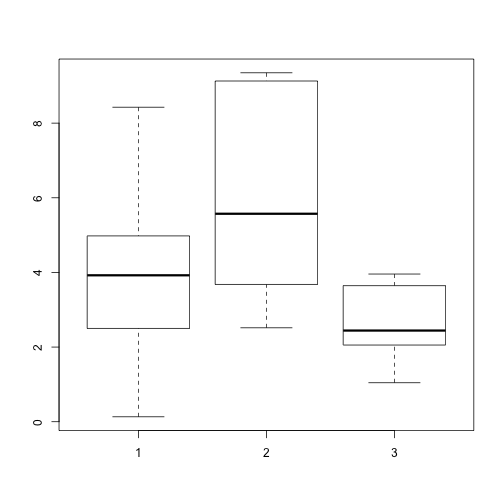
\includegraphics{figure/unnamed-chunk-5-1.png}
\caption{plot of chunk unnamed-chunk-5}
\end{figure}

\begin{Shaded}
\begin{Highlighting}[]
\CommentTok{# generates a stripchart: https://stat.ethz.ch/R-manual/R-devel/library/graphics/html/stripchart.html}
\CommentTok{# one thing is that they require a list}
\CommentTok{# jitter moves the values so they overlap less}
\CommentTok{# try group.names = c("X","Y","Z") as an option}
\KeywordTok{stripchart}\NormalTok{(}\KeywordTok{list}\NormalTok{(x,y,z), }\DataTypeTok{vertical=}\OtherTok{TRUE}\NormalTok{, }\DataTypeTok{method=}\StringTok{"jitter"}\NormalTok{, }\DataTypeTok{jitter=}\FloatTok{0.2}\NormalTok{)}
\end{Highlighting}
\end{Shaded}

\begin{figure}[htbp]
\centering
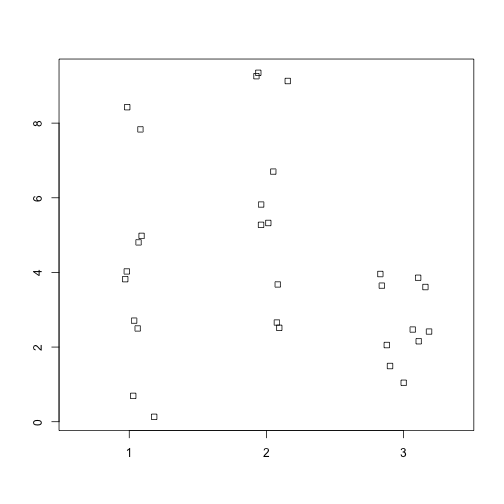
\includegraphics{figure/unnamed-chunk-5-2.png}
\caption{plot of chunk unnamed-chunk-5}
\end{figure}

make sure you have the ability to generate and save R markdown documents
for next class

for your exploration:

\begin{itemize}
\item
  what is the dimension of xyz as a data.frame or a matrix?
\item
  can you tell the difference between the rnorm and runif outputs for
  n=3, n=10, n=100?
\item
  what is the difference between these three subset forms?
\end{itemize}

-- df.xyz\$z{[}1:5{]}

-- df.xyz{[}1:5,3{]}

-- xyz{[}1:5,``z''{]}

\end{document}
